\section{Simulations}

For an internal calibration of the LUX detector to be successful two conditions had to be met.  First, there must be enough events detected during the calibration to accurately measure the tritium spectrum.  We chose to define a factor of 100 over the number of  background events which LUX collects over 300 days to be a sufficient number of CH$_3$T decays for the calibration.  The nominal background rate of LUX is $8.4 \times 10^{-4} \frac{events}{keV*kg*day}$.  Since the fiducial volume of LUX is 100 kg, and the energy spectrum of interest ranges from 1.3 keV to 8 keV, we expect 170 background events in LUX over 300 days.  Thus, we set a goal of collecting around 17,000 events during our CH$_3$T calibration.  The second condition for a successful CH$_3$T calibration is that any residual CH$_3$T remaining after purification must not add a significant contribution to the background rate in the detector.  We chose to define the tolerable CH$_3$T activity after a calibration to be 5\% of the nominal background rate in LUX, setting a limit on the residual CH$_3$T activity of $8.4 \times 10^{-4} \frac{events}{keV*kg*day} \times 100 \; kg \times 6.7 \; keV \times \frac{1 \; day}{86400 \; sec} \times 0.05 = 0.33 \mu Bq$.

To achieve these goals we had to determine how much initial CH$_3$T activity to inject into LUX by numerically modeling the purification and residual diffusion of CH$_3$T in LUX.  Fick's two laws are simple differential equations which describe the diffusion process.  The first law describes the flux of a material through a surface.  Its general form is given by
\[J=-D \nabla \phi,\]
where $J$ is the amount of material per unit area per unit time, $D$ is the diffusion coefficient, and $\phi$ is the concentration function of the material. Combining this with the continuity equation,
\[\frac{\delta\phi}{\delta t} + \nabla \cdot J =0,\]
which states that a change in density in any part of the system is due to inflow and outflow of material results in Fick's second law,
\[\frac{\delta \phi}{\delta t} = D \nabla^2\phi,\]
which describes the transport of a material by diffusion.

To implement these diffusion laws into our model we must determine the diffusion coefficient of CH$_3$T in the plastics of LUX.  At room temperature, the diffusion coefficient of methane in Teflon is measured to be $2.3 \times 10^{-7} \frac{cm^2}{sec} $. \cite{Miyake}  The temperature dependence of this diffusion constant is modeled by the Arrhenius equation,
\[D=Ae^{\frac{-E_a}{RT}},\]
where $E_a$ is the activation energy, $R$ is the gas constant, and $T$ is the temperature.  This suggests an adjustment factor to the diffusion constant of $10^{-6}$ at liquid xenon temperature.  This adjustment factor is equivalent to increasing the thickness of the plastic in our model by a factor of 1,000.  For this reason we are motivated to use half-infinite line boundary conditions in our diffusion model.

\newcommand*{\Scale}[2][4]{\scalebox{#1}{$#2$}}%

The analytic solution to Fick's second law using half-infite line boundary conditions is
\[\Scale[0.5]{\phi (x,t) = KC_{out} - \int \limits_0^t erf(\frac{x}{\sqrt{4D(t - \tau)}})K\dot{C_{out}}(\tau)d\tau - KC_{out}(0)erf(\frac{x}{\sqrt{4Dt}}),}\]
where $K$ is the solubility of the material and $C_{out}$ is the outside concentration of the material. \cite{Piche} For the outgassing process we are only interested in the flux of material out of the plastic.  This is given by Fick's first law evaluated at $x=0$,
\[J_{out}(t)= - K \sqrt{\frac{D}{\pi}}( \int \limits_0^t \frac{\dot{C_{out}}(\tau)}{\sqrt{t-\tau}} d \tau + \frac{C_{out}(t)}{\sqrt{t}}),\]
where the sign has been flipped since the flux of material is outward.  We see that it is no longer possible to evaluate $K$ and $D$ separately, since the diffusion in and out of the plastic is completely determined by the time-dependent concentration outside of the plastic.  To simplify our model, we define a new constant
\[ G = K \sqrt{ \frac{D}{ \pi }} .\]


\subsection{Outgassing Experiments}

To determine the value of G for our simulations we surrounded the PMTs in our liquid phase R\&D experiment with polyethylene or teflon panels during some of our data sets.  The experimental procedure for these data sets was to collect an adequate amount of background data, inject CH$_3$T into the liquid xenon, wait for the CH$_3$T event rate to plateau, purify the CH$_3$T away until we reached the initial background event rate, then bypass the purifier on our system to study outgassing effects.  Once the purifier had been bypassed we discovered two sources of residual CH$_3$T contamination.  

\begin{figure}[h]
\centering
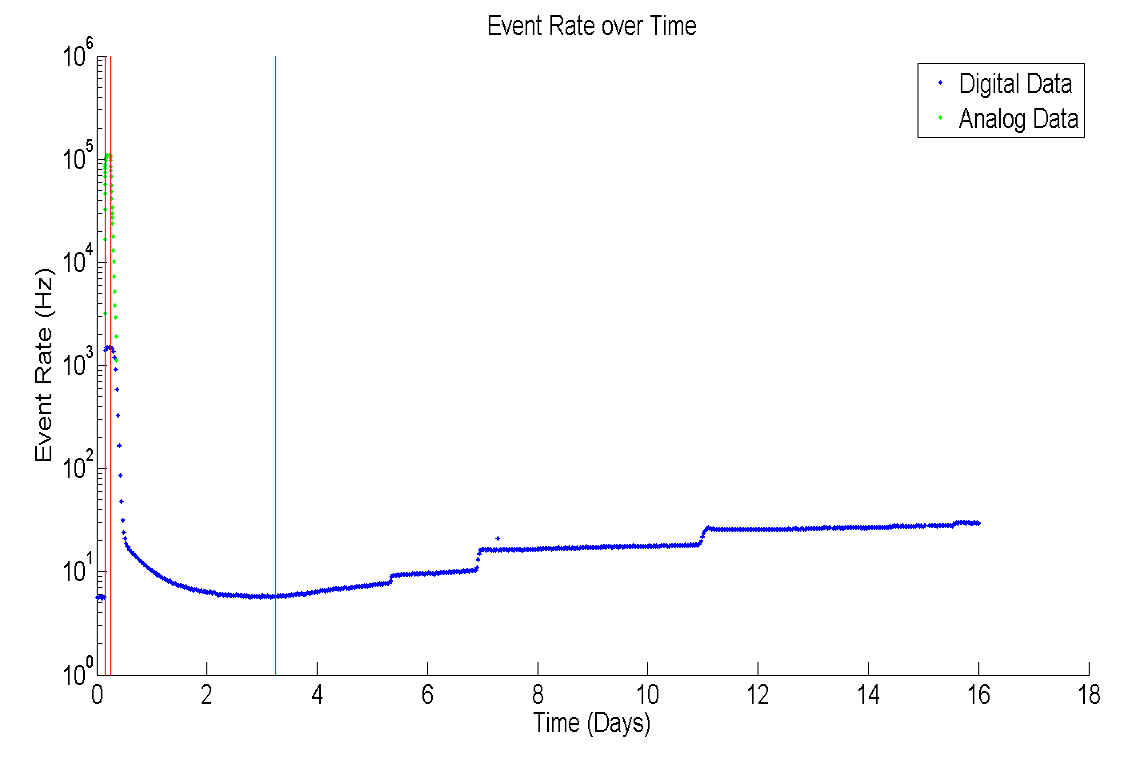
\includegraphics[scale=0.2]{Outgassing_TimeHisto_Log.png}
\caption{A time histogram of the CH$_3$T rate in our system.  The third red line indicates when our purifier was bypassed.}
\label{fig:OutGas}
\end{figure}

We see a gradual rise in CH$_3$T activity after bypassing our purifier due to outgassing of CH$_3$T from the plastic panels.  This outgassing effect will be discussed in detail in Section 4. In addition to this steady rise, we see large steps in CH$_3$T activity at random intervals.  These step features occur every ~3 days on average.  The longest period of time without a step occurring was 5.08 days. To examine these step features more closely, we analyzed the spectra from one of these events.  We found that the integral of the spectra rose from 8833 $\pm$ 93.98 to 17190 $\pm$ 131.11 during the event, a increase of 194.6\%. 

\begin{figure}[h]
\centering
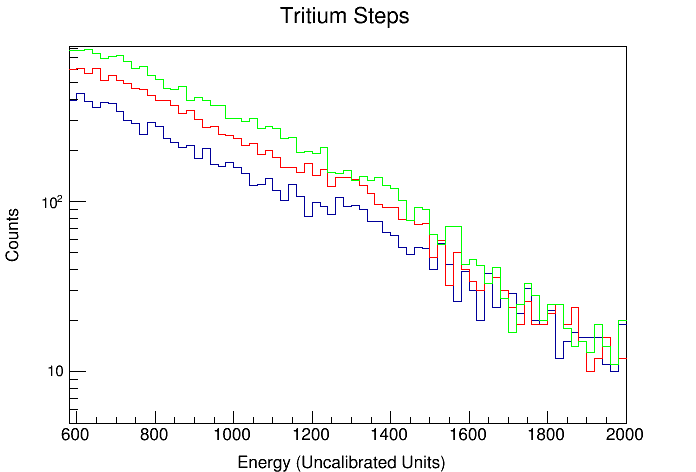
\includegraphics[scale=0.25]{Steps_Overlay.png}
\caption{An overlay of three spectra from a step in CH$_3$T after bypassing our purifier.  The blue spectrum was collected prior to a step occurring, the red spectrum was collected while a step was occurring, and the green spectrum was collected after the step had reached a plateau.}
\label{fig:Steps}
\end{figure}

Such an increase in CH$_3$T activity can be produced through two mechanisms -- a drift in PMT gain which would shift the CH$_3$T spectrum horizontally, or an increase in CH$_3$T activity shifting the CH$_3$T spectrum vertically.  To determine if our PMT gain was shifting during our CH$_3$T data sets we used an external Cesium-137 to a construct time histogram of the Cesium-137 rate.  Over eight days the Cesium-137 event rate remained flat, with an initial event rate of 120255 $\pm$ 346.778 (observed Bq) and a final event rate of 115469 $\pm$ 339.807 (observed Bq). We conclude that the rise in tritium rate during the step events can not be due to our PMT gain drifting, and must therefore be a result of an increase in the amount of CH$_3$T in the fiducial region of our detector.  We suspect this increase in CH$_3$T is due to pockets of stagnant gas slowly moving into the detector's fiducial region.  To avoid such a source of residual CH$_3$T contamination, a detector wishing to using tritiated methane as an internal calibration source must be designed such that no areas of stagnant gas exist within its system.

\begin{figure}[h]
\centering
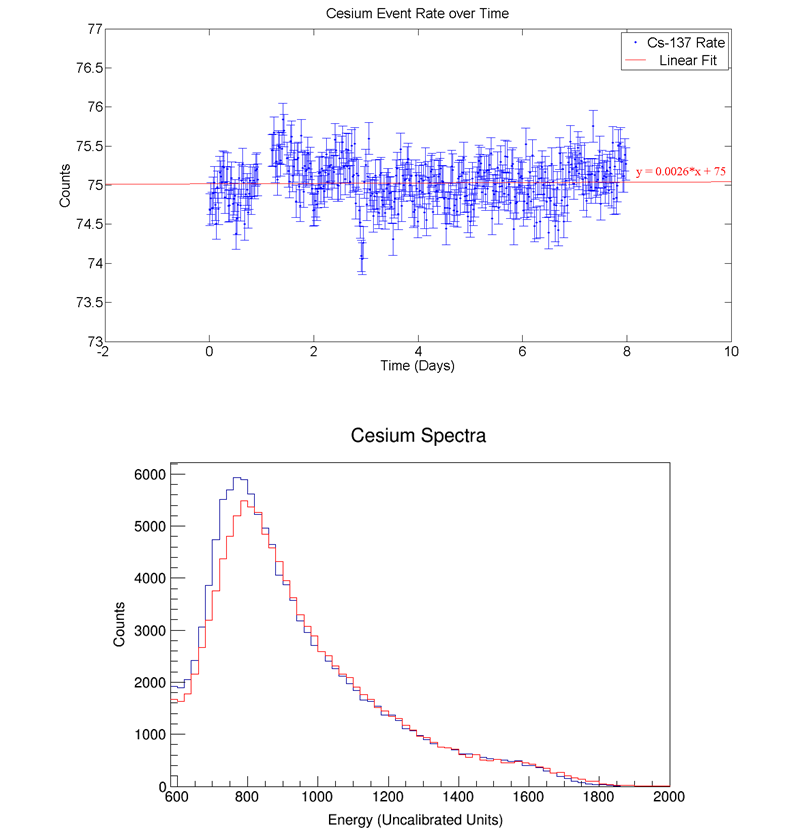
\includegraphics[scale=0.3]{Cesium_Combined_Fit.png}
\caption{Top: A time histogram of Cesium-137 events in our detector. Bottom: An overlay of the initial and final Cs-137 spectrum from above.}
\label{fig:CsFit}
\end{figure}

We can fit the integral of our equation for the flux out of the plastic over time to the outgassing data collected in Maryland's liquid xenon system to extract a value for the constant $G$. Since these outgassing data includes step features from stagnant pockets of unpurified CH$_3$T, we can set an upper limit on $G$ by assuming the step features are a result of outgassing itself, and a lower limit on $G$ by subtracting the steps out of our data, treating them as if they have no connection to outgassing at all. With this method we loosely constrain $0.001 \; \frac{cm}{\sqrt{day}} \leq G \leq 0.01 \; \frac{cm}{\sqrt{day}}.$ 

\begin{figure}[H]
\centering
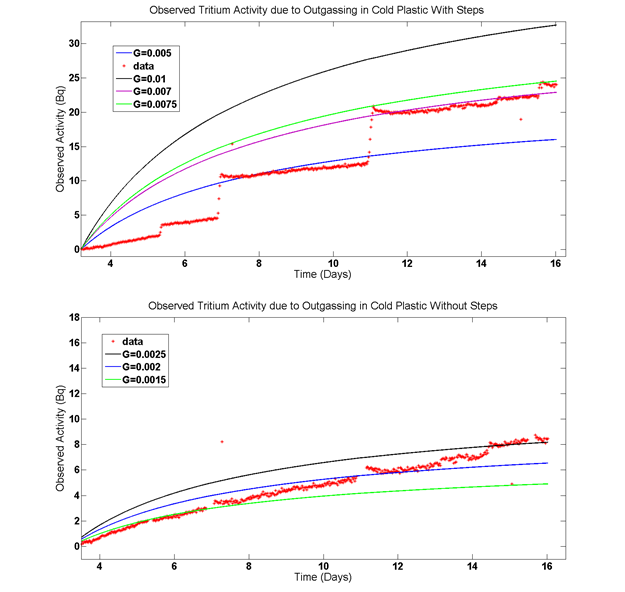
\includegraphics[scale=0.4]{StepsandNoSteps.png}
\caption{Top: A fit of the integral of the flux of CH$_3$T out of plastic over time assuming that the step features are due to diffusion.  This fit is used to set an upper limit on $G$.  Bottom: A fit of the integral of the flux of CH$_3$T out of plastic over time assuming that the step features are not due to diffusion.  This fit is used to set a lower limit on $G$. }
\label{fig:StepsFit}
\end{figure}

\subsection{Implications for LUX}

With a constraint on $G$ taken from the analytic solution to Fick's second law, we turn to numerical simulation to answer the question of how much initial CH$_3$T activity to inject into LUX to meet our calibration conditions.  Several assumptions are made to simplify the numerical model.  First, we approximate the diffusion into plastic as being a one dimensional process. In three dimensions, Fick's laws are
\[J=-D\nabla \phi\]
\[\frac{\delta\phi}{\delta t} = D \nabla^2 \phi .\]
In cylindrical coordinates, these equations become
\[J = -D (\frac{\delta \phi}{\delta r} \vec{r} + \frac{1}{r}\frac{\delta \phi}{\delta \theta}\vec{\theta} + \frac{\delta \phi}{\delta z}\vec{z})\]
\[\frac{\delta \phi}{\delta t} = D ( \frac{\delta^2\phi}{\delta r^2} + \frac{1}{r}\frac{\delta \phi}{\delta r} + \frac{1}{r^2}\frac{\delta^2 \phi}{\delta \theta^2} + \frac{\delta^2 \theta}{\delta z^2}).\]
Since the plastic in our detector at Maryland and in LUX can be approximated by a cylindrical shell, there is no dependence on the azimuthal or $z$ coordinates.  Since $r$ is large compared to the thickness of the plastic shell, $\frac{\delta^2 \phi}{\delta r^2} \gg \frac{1}{r} \frac {\delta \phi}{\delta r}$, so we can make the approximations
\[J=-D\frac{\delta \phi}{\delta r}\vec{r}\]
\[\frac{\delta \phi}{\delta t} = D \frac{\delta^2 \phi}{\delta r^2}.\]  We assume the concentration of CH$_3$T in LUX is uniform throughout its volume.  This assumption is justified, since the design of LUX creates currents which stir the liquid xenon.  With perfect mixing the effect of the purifier can be modeled by adding an exponential time dependence to the outer volume.  The time constant of this decay is equal to the time it takes xenon to recircculate through the LUX detector.

We use a simple implementation of the first order Euler method for our numerical simulations.  The finite difference approximations of Fick's two laws in one dimension are 
\[J_{i,j} = -D \frac{\phi_{i+1,j}-\phi_{i,j}}{\Delta x }\]
\[\phi_{i,j+1} = \phi_{i,j} + \Delta t (D \frac{\phi_{i+1,j} - 2 \phi_{i,j} + \phi_{i-1,j}}{\Delta x^2}),\]
where $i$ is the spacial index and $j$ is the time index.  To avoid divergent solutions, we must have
\[D \frac{\Delta t}{\Delta x^2} \leq \frac{1}{2}.\]
For effects to be propagated across $N$ spacial bins, $N$ time steps are required.  Therefore, the effective time resolution is
\[\Delta t_{effective} = \Delta t \times N_x.\]

The diffusion is simulated by setting the concentration at the boundary of the piece equal to $KC_{out}$, where $C_{out}$ is the concentration of CH$_3$T in the xenon.  This concentration is dependent on time according to
\[\frac{\delta C_{out}}{\delta t} = J_{out} \frac{A_{plastic}}{V_{xenon}}-\frac{C_{out}}{\tau},\]
where $A_{plastic}$ is the surface area of the plastic cylinder, $V_{xenon}$ is the total volume of xenon in the fiducial region, and $\tau$ is the time it takes for one full purification cycle.  The first term on the right of this equation models outgassing of CH$_3$T from the plastic cylinder, while the second term models removal of CH$_3$T through purification.  Using the first order Euler method, we arrive at an expression for $C_{out}$ given by
\[C_{j+1}=C_j + \Delta t [(J_{1,j}-J_{N_x,j})\frac{A_{plastic}}{V_{xenon}}-\frac{C_j}{\tau}].\]
The initial concentration is defined by dividing the desired injection activity by the volume of the fiducial region.  We choose $D = 2.3 \times 10^{-9} \frac {cm^2}{sec}$ such that the half-infinite boundary conditions in our diffusion model is valid, and combine this with our allowed range of values for $G$ to extract a value for $K$.  We find that for all $G$ values in our allowed range, an initial injection activity of 0.1 Bq results in 15,000 calibration events with the background rate returning to $<$ 5\% of its initial value in less than one month. 

\begin{figure}[H]
\centering
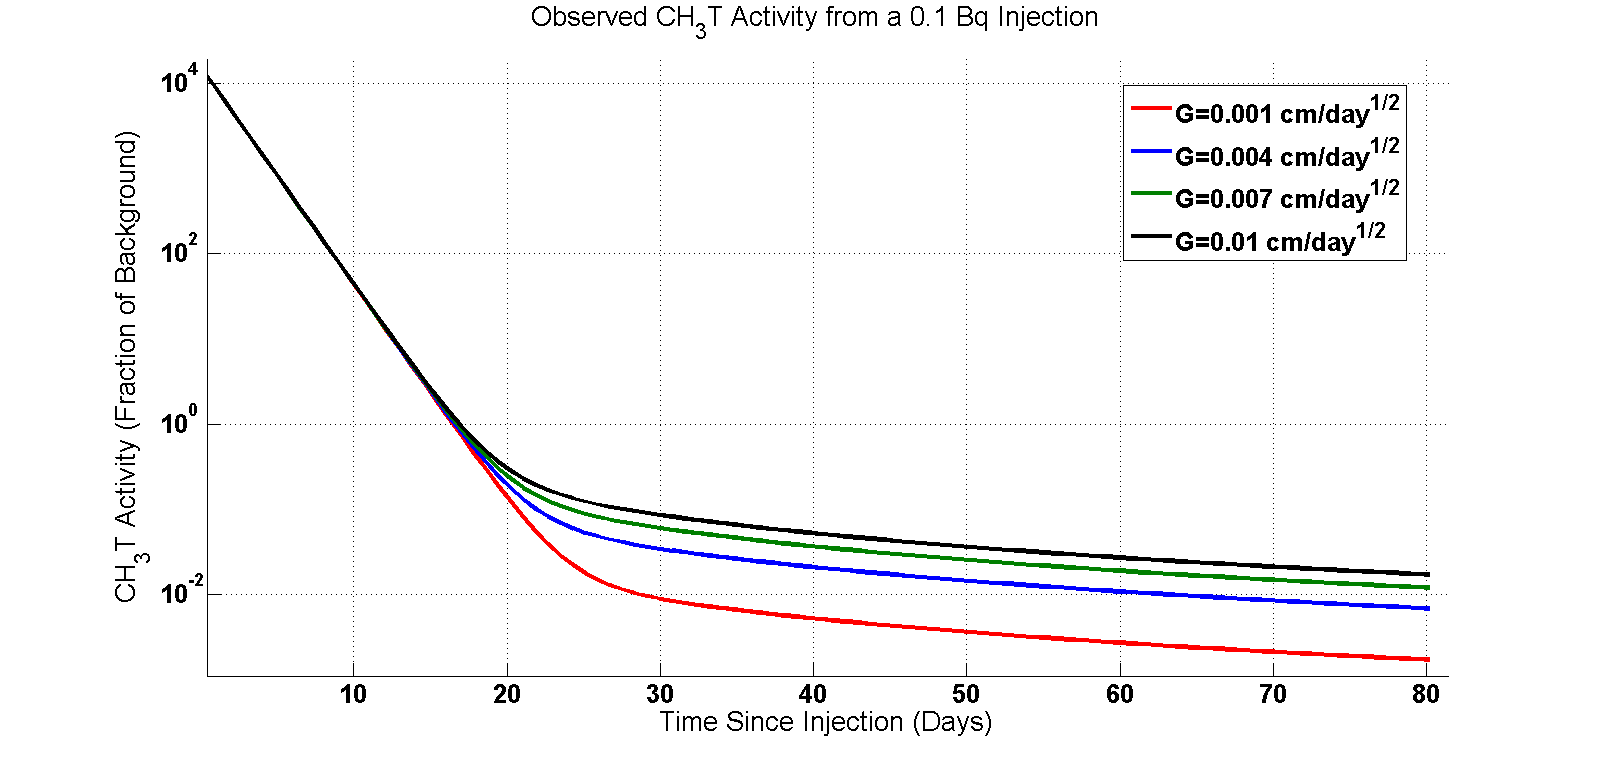
\includegraphics[scale=0.15]{LUXActivityOverTime.png}
\caption{Simulated activity over time in LUX after a 0.1 Bq injection.}
\label{fig:LUXActivity}
\end{figure}

NOTE: UPDATE THIS SECTION, REDO EVERYTHING WITH SAME FIDUCIAL VOLUMES, TIME CONSTANTS, ETC
